\documentclass[tikz,border=4pt]{standalone}
% Estilo común de los diagramas de bloques (se usa con \input en cada standalone)
\usepackage[defaultsans,scale=0.92]{lato}
\usepackage{libertinust1math}
\usepackage{xcolor,amsmath}
\usepackage{tikz}
\usetikzlibrary{positioning,arrows.meta,calc,shapes.geometric}
\usepackage{../../notacion}
\definecolor{ctrlazul}{HTML}{1E5AA8}\definecolor{ctrlnoche}{HTML}{14213D}
\definecolor{ctrlcoral}{HTML}{D1495B}\definecolor{ctrlverde}{HTML}{2A9D8F}
\definecolor{ctrlambar}{HTML}{E09F3E}\definecolor{ctrlgris}{HTML}{5C677D}
\definecolor{ctrlvioleta}{HTML}{6C4AB6}\definecolor{ctrlteal}{HTML}{0F7173}
\tikzset{
  >={Stealth[length=2.4mm]}, every node/.style={font=\small},
  bloque/.style={draw=ctrlnoche,fill=ctrlazul!7,thick,rounded corners=1.5pt,minimum height=9mm,minimum width=13mm,inner sep=4pt},
  suma/.style={draw=ctrlnoche,thick,circle,inner sep=0pt,minimum size=6mm},
  senal/.style={->,thick,draw=ctrlnoche},
  rot/.style={font=\footnotesize,text=ctrlgris},
}

\begin{document}
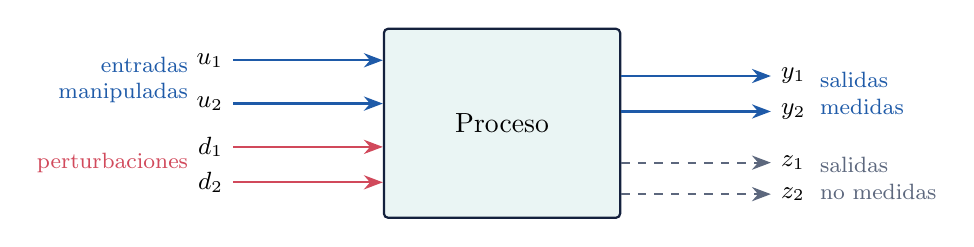
\begin{tikzpicture}
  \node[bloque,fill=ctrlverde!10,minimum width=30mm,minimum height=24mm,font=\normalsize] (p) {Proceso};
  \foreach \y/\t in {0.55/{$u_1$},0/{$u_2$}}{\draw[senal,draw=ctrlazul] ($(p.west)+(-1.9,\y+0.25)$)--($(p.west)+(0,\y+0.25)$) node[pos=0,left]{\t};}
  \foreach \y/\t in {-0.55/{$d_1$},-1.0/{$d_2$}}{\draw[senal,draw=ctrlcoral] ($(p.west)+(-1.9,\y+0.25)$)--($(p.west)+(0,\y+0.25)$) node[pos=0,left]{\t};}
  \foreach \y/\t in {0.6/{$y_1$},0.15/{$y_2$}}{\draw[senal,draw=ctrlazul] ($(p.east)+(0,\y)$)--($(p.east)+(1.9,\y)$) node[right]{\t};}
  \foreach \y/\t in {-0.5/{$z_1$},-0.9/{$z_2$}}{\draw[senal,draw=ctrlgris,dashed] ($(p.east)+(0,\y)$)--($(p.east)+(1.9,\y)$) node[right]{\t};}
  \node[align=right,font=\footnotesize,text=ctrlazul,anchor=east] at ($(p.west)+(-2.35,0.55)$) {entradas\\manipuladas};
  \node[align=right,font=\footnotesize,text=ctrlcoral,anchor=east] at ($(p.west)+(-2.35,-0.5)$) {perturbaciones};
  \node[align=left,font=\footnotesize,text=ctrlazul,anchor=west] at ($(p.east)+(2.4,0.38)$) {salidas\\medidas};
  \node[align=left,font=\footnotesize,text=ctrlgris,anchor=west] at ($(p.east)+(2.4,-0.7)$) {salidas\\no medidas};
\end{tikzpicture}
\end{document}
